\documentclass[11pt]{article}

\usepackage[margin=1in]{geometry}
\usepackage{graphicx}
\usepackage{float}
\usepackage{pdflscape}
\usepackage{booktabs}
\usepackage{tabularx}
\usepackage{enumitem}
\usepackage{caption}
\usepackage[hidelinks]{hyperref}

\graphicspath{{figures/}{DesignModelsFall2026/figures/}}
\captionsetup{font=small, labelfont=bf}
\setlist{itemsep=2pt, topsep=4pt}
\newcommand{\project}{\textit{People of the Holocaust}}
\newcommand{\ecg}{\textit{Encyclopedia of Camps and Ghettos}}

\begin{document}

% ---------------------------------------------------------------- title page
\begin{titlepage}
  \centering
  \vspace*{\fill}
  {\LARGE\bfseries People of the Holocaust\par}
  \vspace{1.2em}
  {\Large\bfseries System Design Models\par}
  \vspace{2.5em}
  {\Large Marquette University\par}
  \vspace{0.6em}
  {\large COSC 4920 -- Principles of Design\par}
  \vspace{2.5em}
  {\large Version 1.0\par}
  \vspace{0.6em}
  {\large October 19, 2026\par}
  \vspace*{\fill}
\end{titlepage}

\tableofcontents
\listoffigures
\clearpage

% ---------------------------------------------------------------- 1
\section{Introduction}

\subsection{Purpose}
This document collects the design models for the \project{} senior design
project. Each model describes one view of the system: how visitors use the
website, how work flows through the interpreter and the website, how the system
changes state, how the parts communicate over time, how the code is structured,
and how the major components connect. Each diagram is followed by a short
description of what it shows.

\subsection{Scope}
The models cover the three main parts of the system: the Python interpreter that
processes text from the \ecg{} (ECG), the project database that stores the
structured records, and the React and TypeScript website that presents those
records to the public. The database schema is included as a supplementary model.

\subsection{Model Summary}

\begin{table}[H]
  \centering
  \begin{tabularx}{\linewidth}{@{}l X l@{}}
    \toprule
    \textbf{Section} & \textbf{Model} & \textbf{Status} \\
    \midrule
    \ref{sec:usecase}  & UML Use Case Diagram                      & Required \\
    \ref{sec:activity} & UML Activity Diagram                      & Required \\
    \ref{sec:sequence} & UML Sequence Diagram                      & Required \\
    \ref{sec:state}    & UML State Diagram                         & Required \\
    \ref{sec:class}    & UML Class Diagrams (domain and front end) & Required \\
    \ref{sec:block}    & Block Diagram (architecture deliverable)  & Required \\
    \ref{sec:schema}   & Database Schema                           & Supplementary \\
    \bottomrule
  \end{tabularx}
  \caption{Design models included in this document}
\end{table}

% ---------------------------------------------------------------- 2
\clearpage
\section{UML Use Case Diagram}\label{sec:usecase}

The use case diagram shows what a visitor can do on the public website. A single
actor, the website visitor, is connected to nine use cases. No account or login
is involved, so every use case is available to any visitor.

\begin{itemize}
  \item \textbf{Project information:} read the project background.
  \item \textbf{People:} browse people, search people by name, and view a
        person's details.
  \item \textbf{Places:} browse places, search places by name, and view a
        place's details.
  \item \textbf{Map:} explore the historical map and view a place's information
        by selecting its marker.
\end{itemize}

\begin{figure}[H]
  \centering
  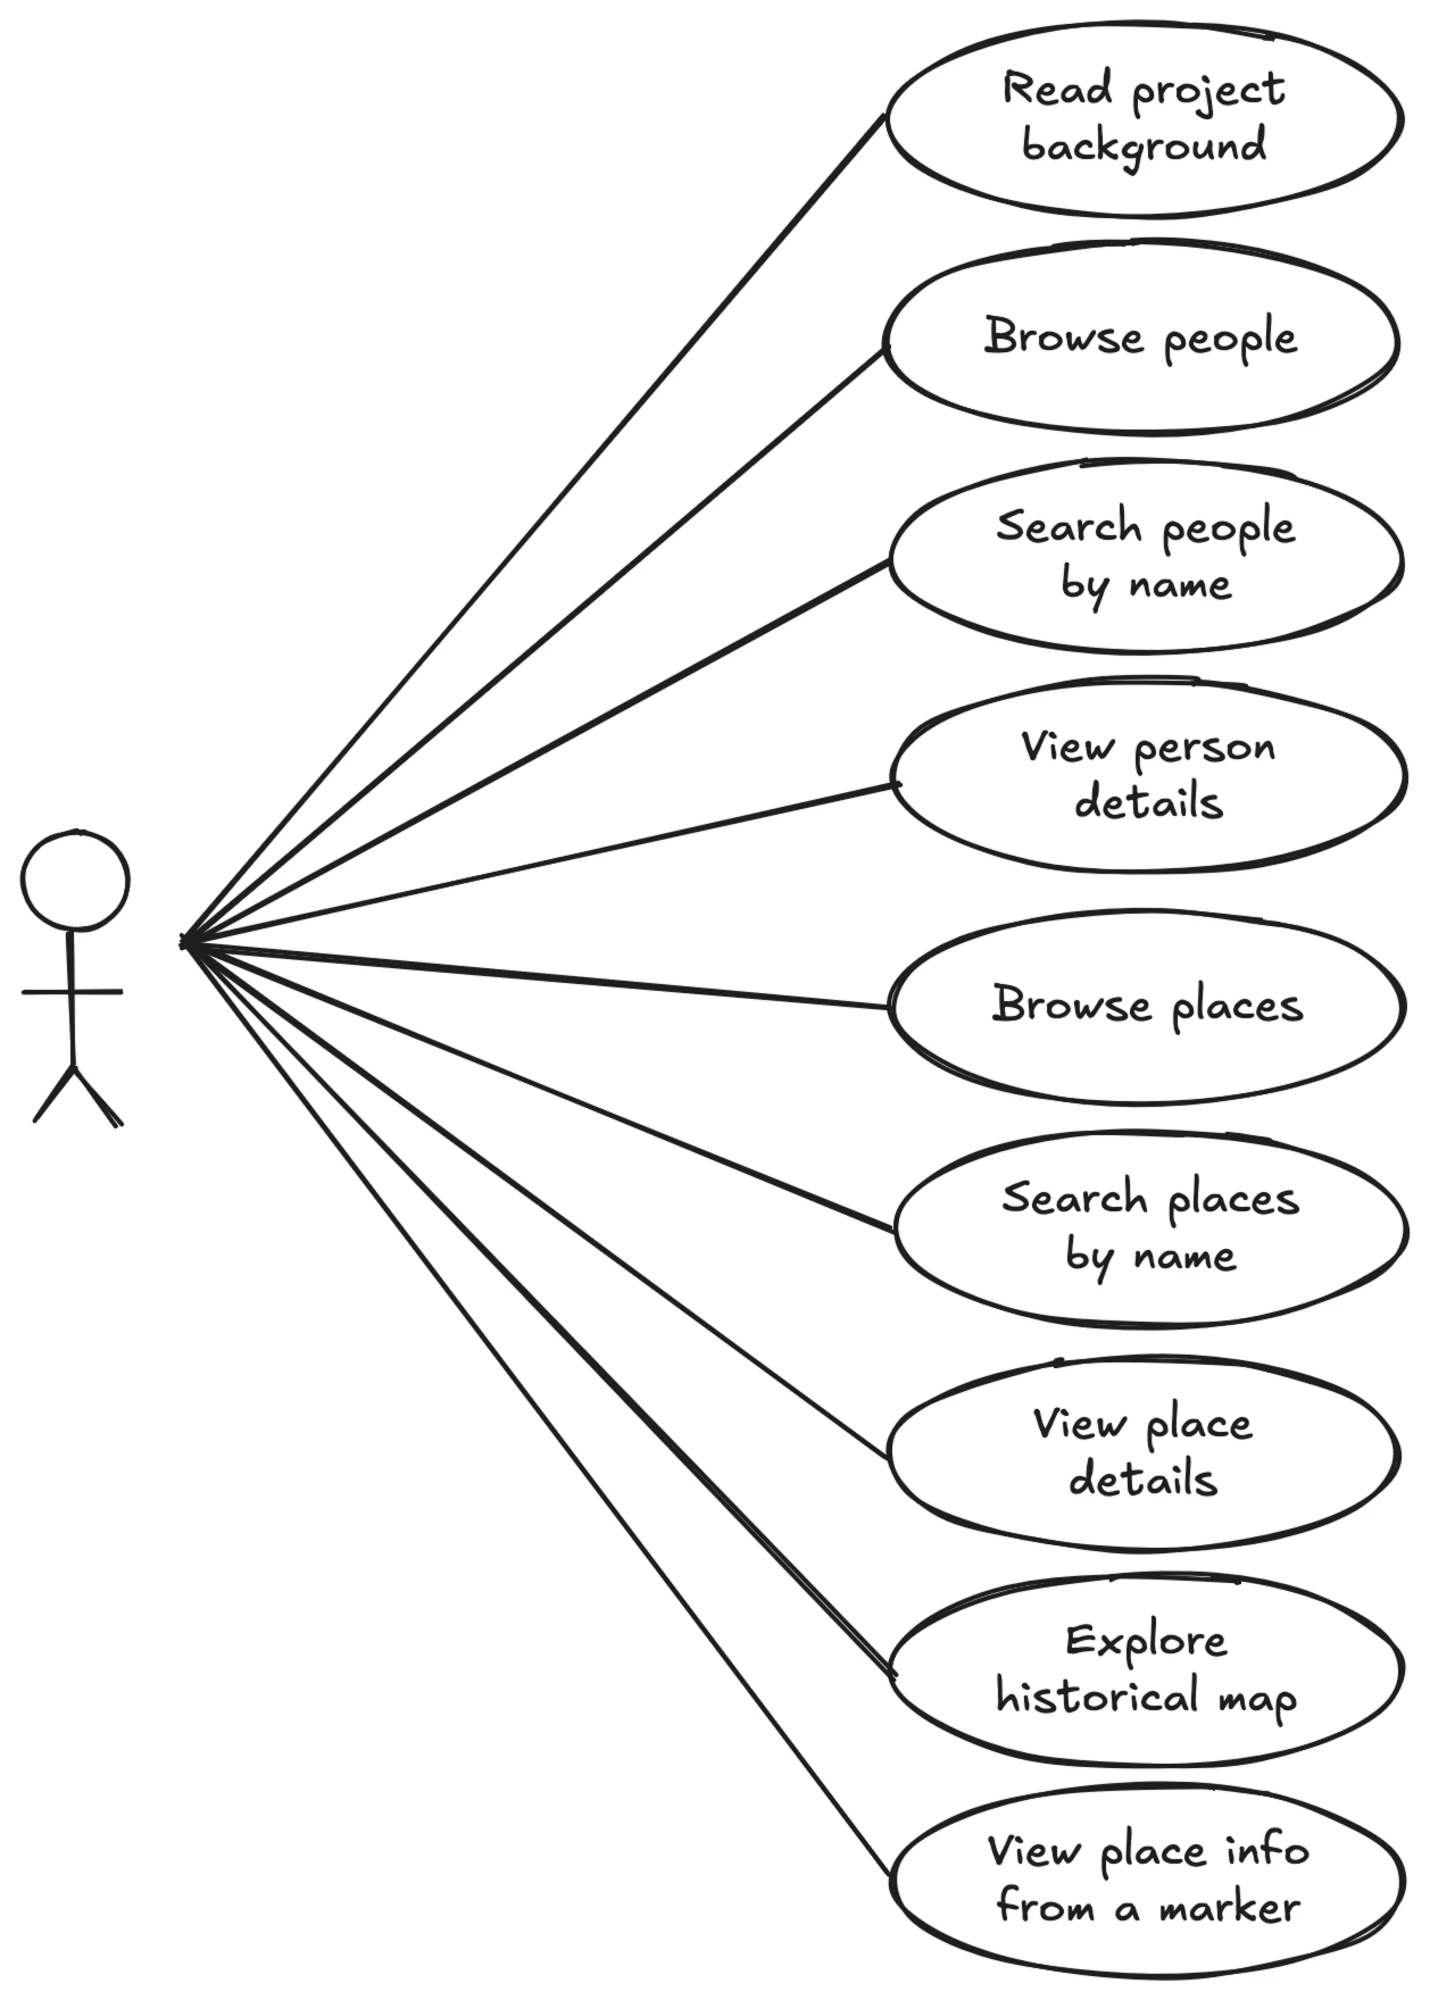
\includegraphics[width=\linewidth,height=0.62\textheight,keepaspectratio]{use-case}
  \caption{Use case diagram for the public website}
\end{figure}

% ---------------------------------------------------------------- 3
\clearpage
\section{UML Activity Diagram}\label{sec:activity}

The activity diagram, titled \textit{System Context Activity Diagram}, follows
two independent flows across four swimlanes: \textit{Project Maintainer},
\textit{PotH System}, \textit{Source Environment}, and \textit{Public Visitor}.
A fork at the start shows that the two flows run separately; as the attached
note states, website access does not depend on an interpreter run completing.

\begin{itemize}
  \item \textbf{Processing flow.} The maintainer initiates source processing.
        The interpreter prepares structured person-name records, then loops
        while source articles remain. For each article, the ECG provides the
        source text and the interpreter retrieves and cleans it. On success, the
        interpreter identifies sentences that contain known people, associates
        activities with people and places, and the database stores the
        processed records with their source context. On failure, the error is
        logged for later review. When no articles remain, the maintainer
        reviews the processing results and error logs.
  \item \textbf{Visitor flow.} The visitor accesses the public website, which
        presents the project background and navigation without a login. The
        visitor chooses what to explore: project background is displayed
        directly, while historical records are supplied by the database and
        presented as records or map locations. Selecting a person, place, or
        map marker displays its related details and context. The visitor
        continues browsing until leaving the website, and both flows join at
        the end.
\end{itemize}

\begin{landscape}
\begin{figure}[p]
  \centering
  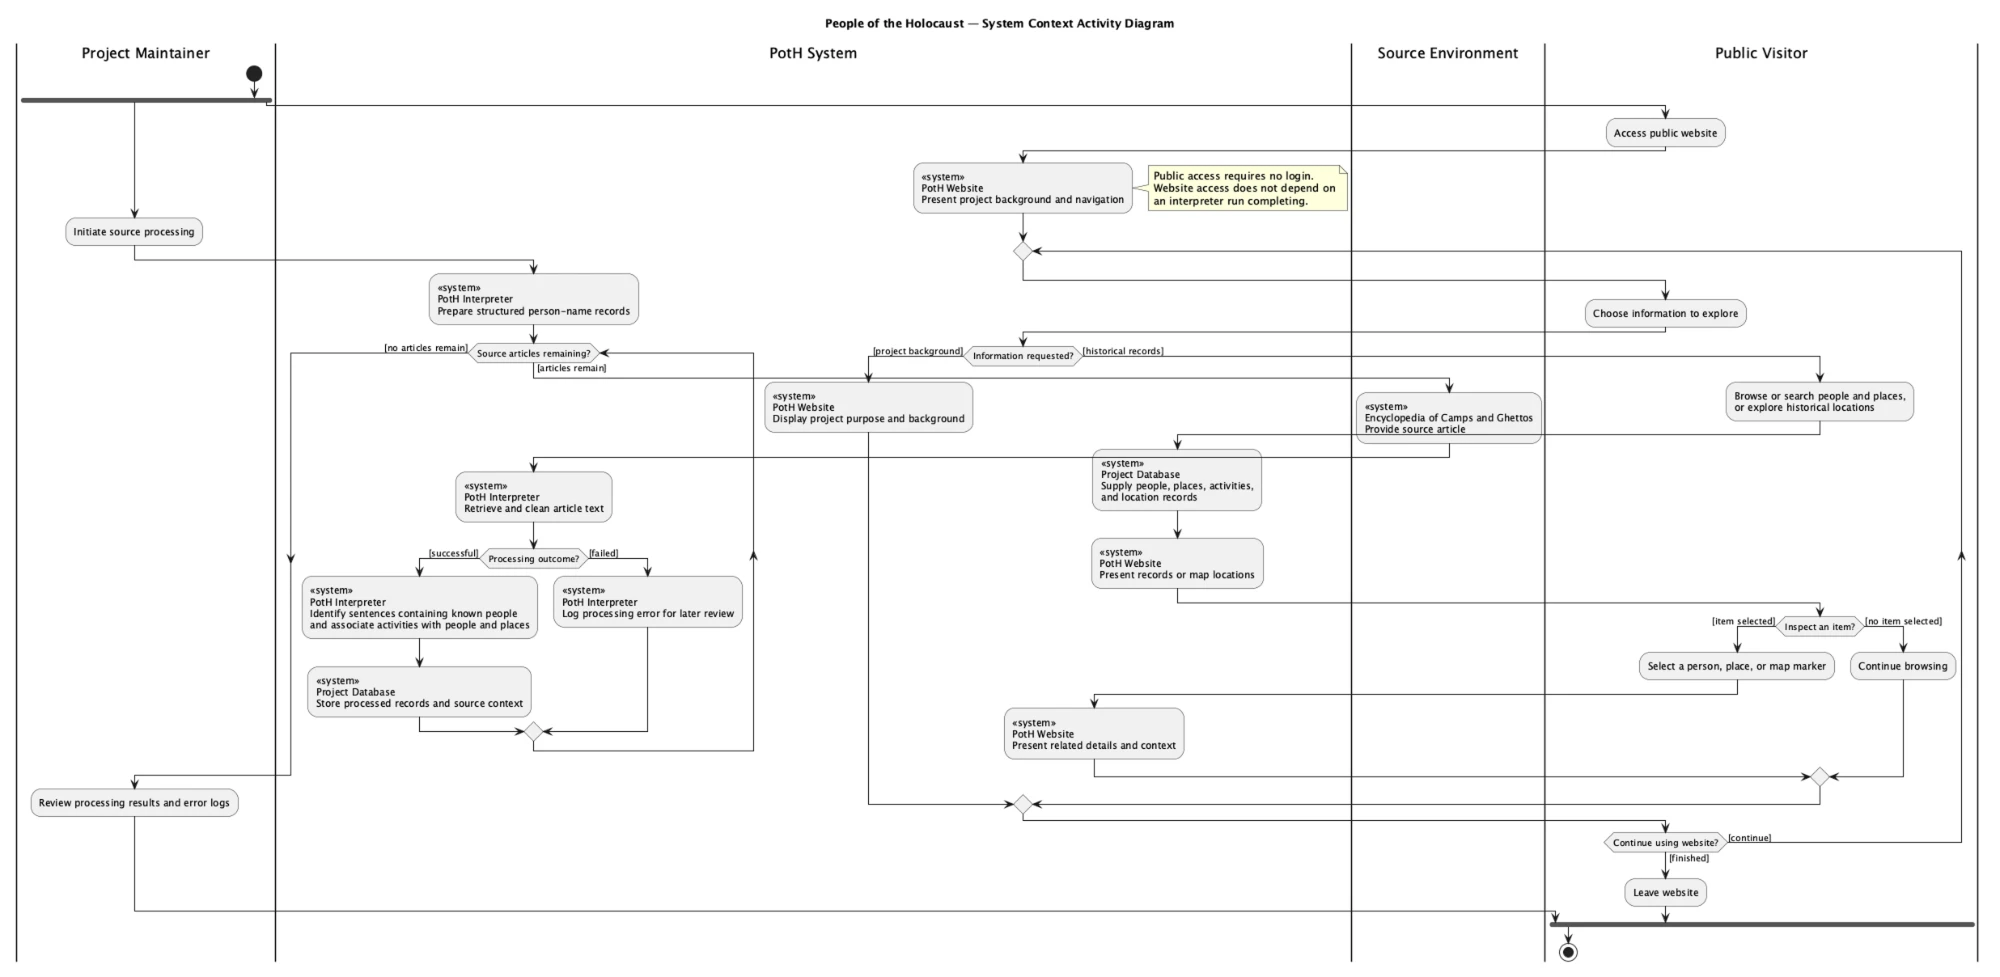
\includegraphics[width=\linewidth,height=0.9\textheight,keepaspectratio]{activity}
  \caption{System context activity diagram}
\end{figure}
\end{landscape}

% ---------------------------------------------------------------- 4
\clearpage
\section{UML Sequence Diagram}\label{sec:sequence}

The sequence diagram shows the messages exchanged between six participants over
time: the NHM Database (the encyclopedia source), the Web Scraper, the NLP
component, the POTH Database, the Frontend, and the User. It is divided into
two frames.

\begin{itemize}
  \item \textbf{Updating Database.} The Web Scraper requests the encyclopedias
        from the source and receives them, stores the response in the POTH
        Database, and receives confirmation. It then passes the entries to the
        NLP component, which stores the resulting NLP tree data in the POTH
        Database and receives confirmation. The Web Scraper and NLP lifelines
        end once their work is complete.
  \item \textbf{User Interaction.} The User opens the homepage and the Frontend
        displays it. When the User submits a query, the Frontend requests the
        necessary information from the POTH Database, receives it, and formats
        and displays it to the User. The Frontend lifeline ends when the User
        closes the session.
\end{itemize}

\begin{figure}[H]
  \centering
  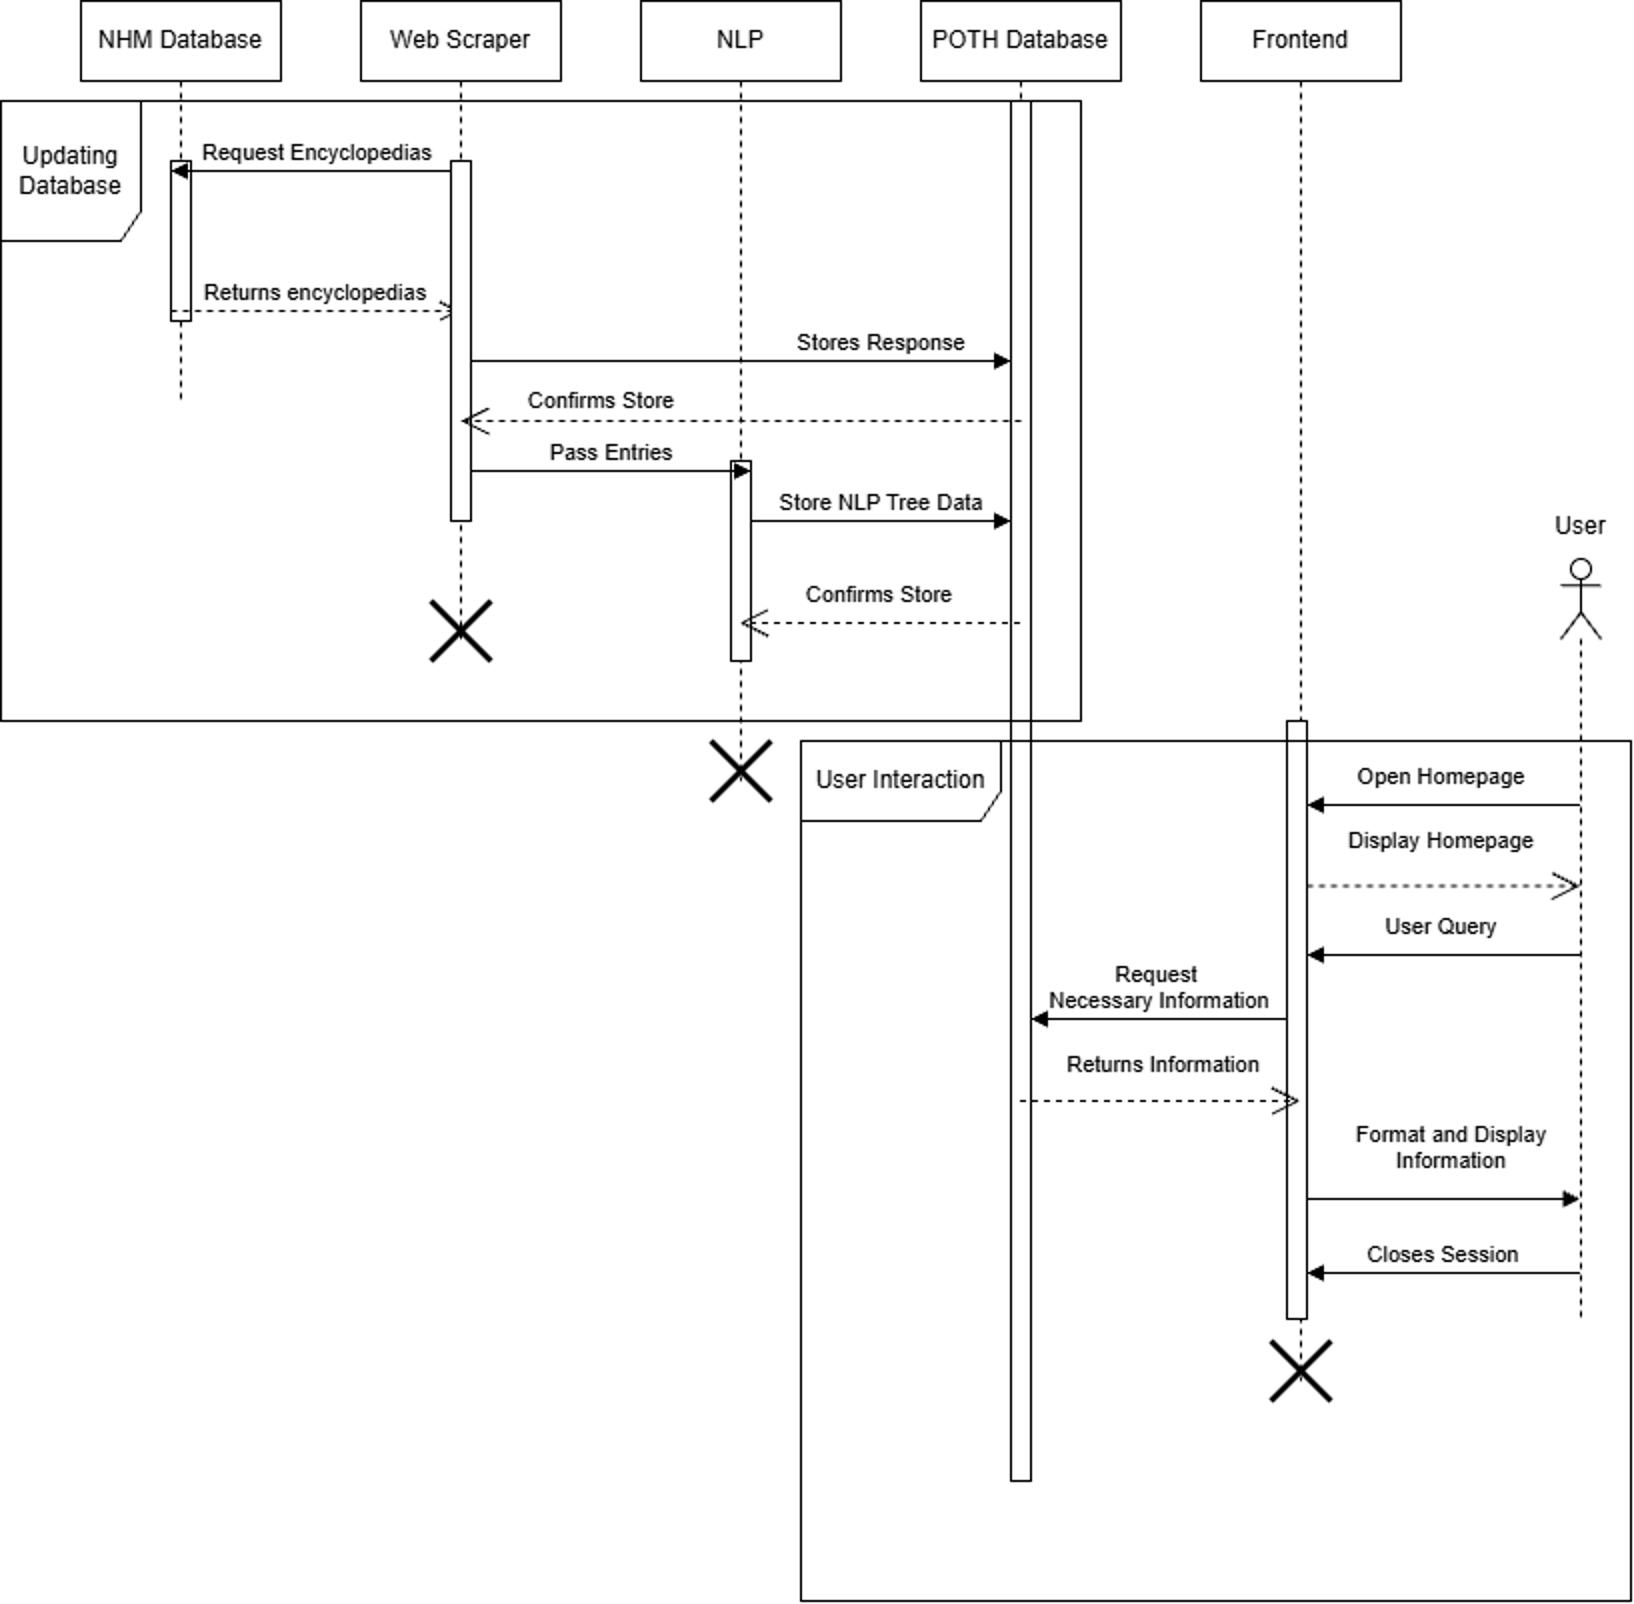
\includegraphics[width=\linewidth,height=0.62\textheight,keepaspectratio]{sequence}
  \caption{Sequence diagram for updating the database and user interaction}
\end{figure}

% ---------------------------------------------------------------- 5
\clearpage
\section{UML State Diagram}\label{sec:state}

The state diagram, titled \textit{System State Diagram}, models the system as a
single \textit{Operational} state containing two concurrent regions:
\textit{Processing} and \textit{Website}.

\begin{itemize}
  \item \textbf{Processing.} The interpreter waits in \textit{AwaitingRun}
        until the maintainer starts a run, then moves to \textit{Preparing}.
        If preparation fails, it enters \textit{Failed} and returns to
        \textit{AwaitingRun} once the issue is resolved. Otherwise it enters
        \textit{Checking}: while articles remain it cycles through
        \textit{Reading}, \textit{Extracting}, and \textit{Storing}, returning
        to \textit{Checking} after each article. A failure while reading,
        extracting, or storing moves to \textit{Logging}, and processing
        continues with the next article once the error is recorded. When no
        articles remain, the run is \textit{Complete} and returns to
        \textit{AwaitingRun} when acknowledged.
  \item \textbf{Website.} The website is \textit{Available} until a visitor
        opens it, starting a \textit{Session} that begins at \textit{Home}.
        From any page the visitor can navigate to \textit{People},
        \textit{Map}, or \textit{Places}. The People and Places states each
        move between a filtered list and a details view, and the Map state
        moves between \textit{Exploring} and \textit{MarkerInfo} when a marker
        is selected or its popup is closed. The session ends when the visitor
        leaves.
\end{itemize}

The notes record that article failures are logged without stopping processing,
that database records persist between runs, that each session represents one
visitor with no authentication, and that missing optional fields do not prevent
details from being viewed.

\begin{landscape}
\begin{figure}[p]
  \centering
  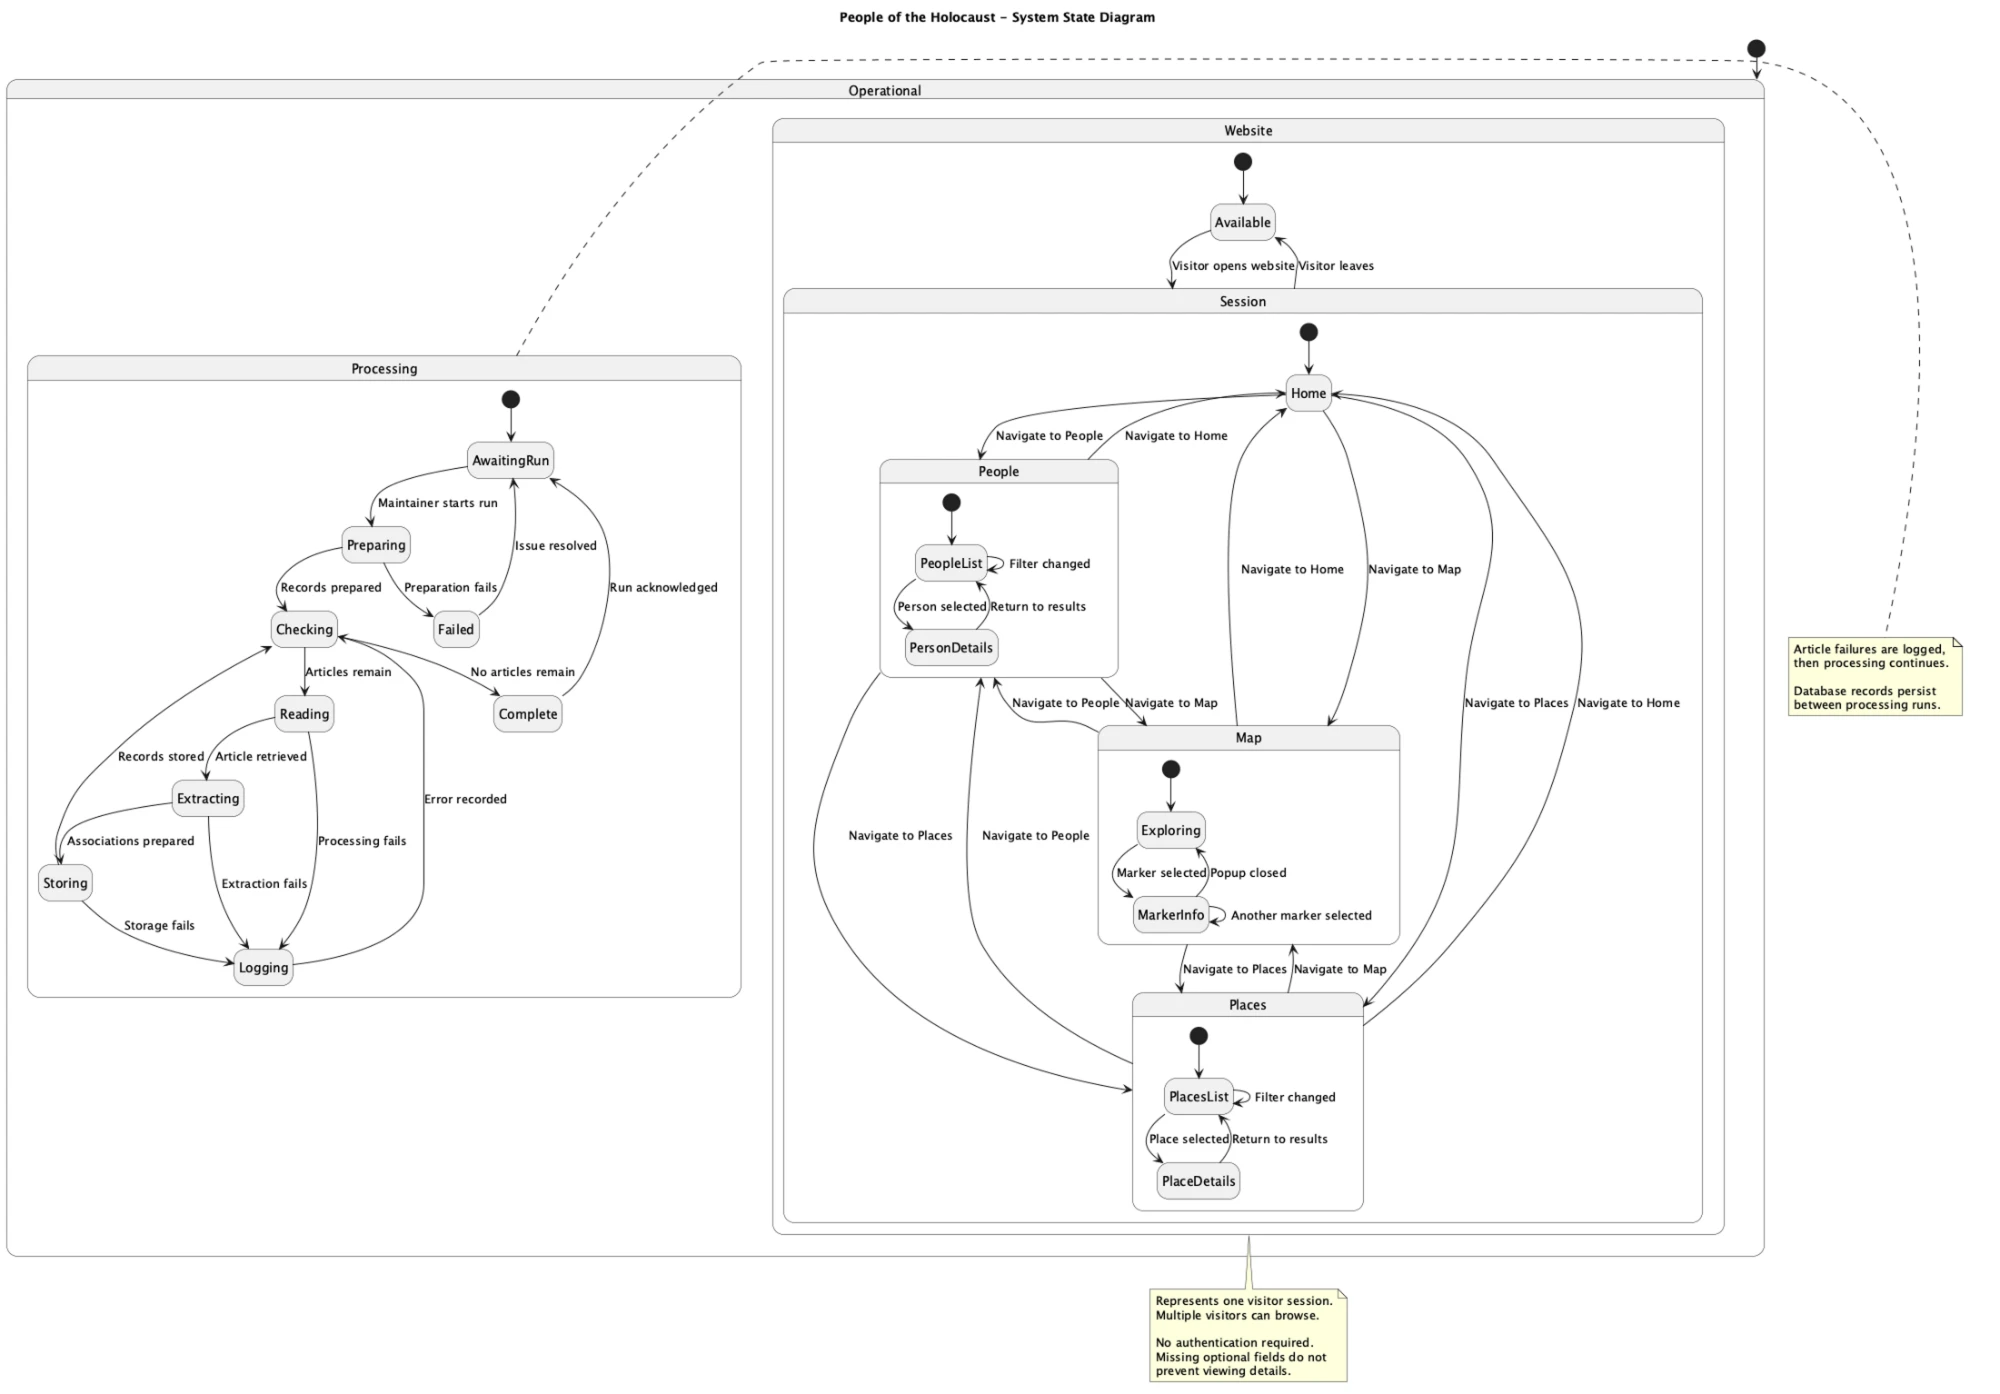
\includegraphics[width=\linewidth,height=0.9\textheight,keepaspectratio]{state}
  \caption{System state diagram}
\end{figure}
\end{landscape}

% ---------------------------------------------------------------- 6
\clearpage
\section{UML Class Diagrams}\label{sec:class}

Two class diagrams describe the structure of the system: a domain model of the
data the system stores, and a model of the front end website.

\subsection{Domain Model}
The domain model shows the encyclopedia's structure and the people and places
drawn from it.

\begin{itemize}
  \item \textbf{Text hierarchy.} A \texttt{Volume} contains many
        \texttt{Article}s, and each \texttt{Article} contains many
        \texttt{Paragraph}s (composition). Each paragraph records its position
        and its start and end pages, so \texttt{citation()} can give the volume
        and page for any quoted text.
  \item \textbf{Mentions.} A \texttt{Paragraph} mentions many \texttt{Person}s
        and many \texttt{Place}s, and each person or place can be mentioned in
        many paragraphs (many-to-many associations).
  \item \textbf{Places.} An \texttt{Article} is about at most one
        \texttt{Place}, which lets each place lead with its own article.
  \item \textbf{People.} Each \texttt{Person} is listed under one or more
        \texttt{NameEntry} records, so alternate spellings of a name refer to
        the same person. A person's kind is given by the \texttt{PersonKind}
        enumeration: Individual, Family, or Brother.
\end{itemize}

\begin{figure}[H]
  \centering
  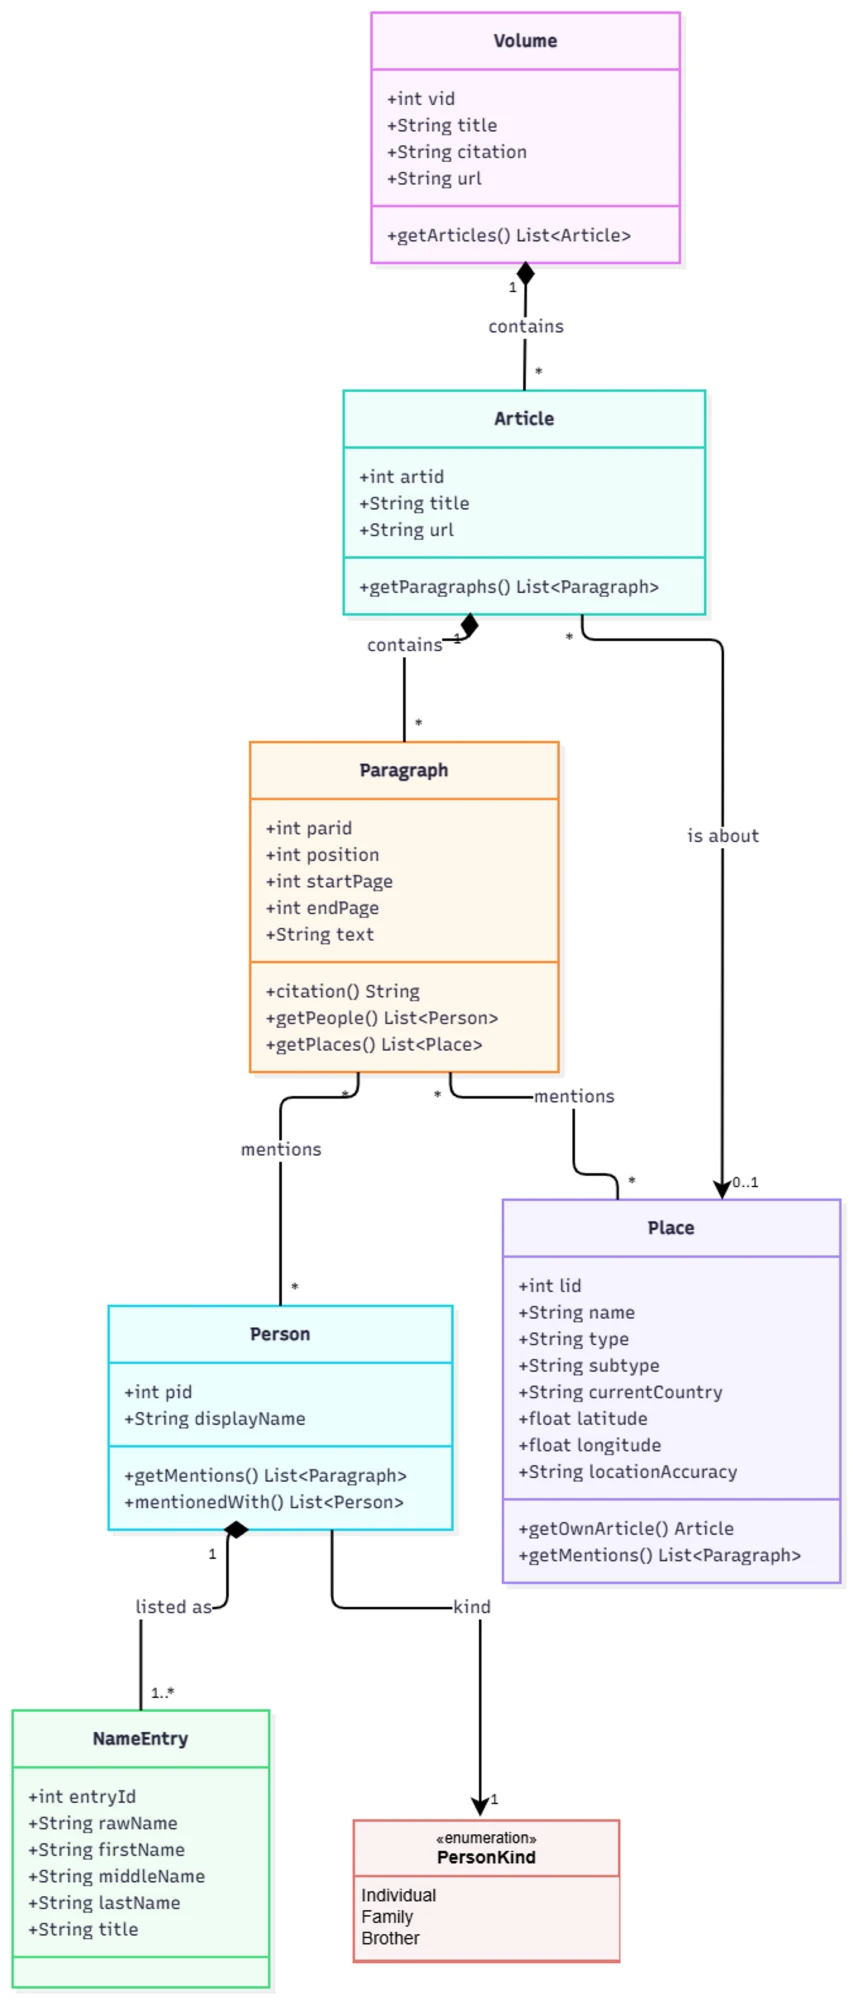
\includegraphics[width=\linewidth,height=0.62\textheight,keepaspectratio]{class-domain}
  \caption{Domain class diagram}
\end{figure}

\clearpage
\subsection{Front End}
The front end class diagram shows the React components of the website and the
data they display.

\begin{itemize}
  \item \textbf{Website and pages.} \texttt{Website} holds the navigation shown
        on every page and is composed of three pages. \texttt{HomePage} presents
        the project and loads no data from the database.
  \item \textbf{People page.} \texttt{PeoplePage} combines a
        \texttt{SearchBar}, a \texttt{PeopleList} of results, and a
        \texttt{PersonDetails} panel shown once a person is selected.
  \item \textbf{Places page.} \texttt{PlacesPage} combines the same
        \texttt{SearchBar}, an interactive \texttt{MapView}, a
        \texttt{PlaceList}, and a \texttt{PlaceDetails} panel. Selecting a
        place from either the map or the list opens its details.
  \item \textbf{Quotes and citations.} Both details panels display a list of
        \texttt{QuoteCard}s. Each card shows one paragraph from the
        encyclopedia with the name highlighted and its citation.
  \item \textbf{Data.} Only \texttt{DataLoader} retrieves data. The
        \texttt{<<type>>} classes describe the
        shape of the data it returns, with \texttt{Quote} holding a
        paragraph's text, volume, article, and pages.
\end{itemize}

\begin{figure}[H]
  \centering
  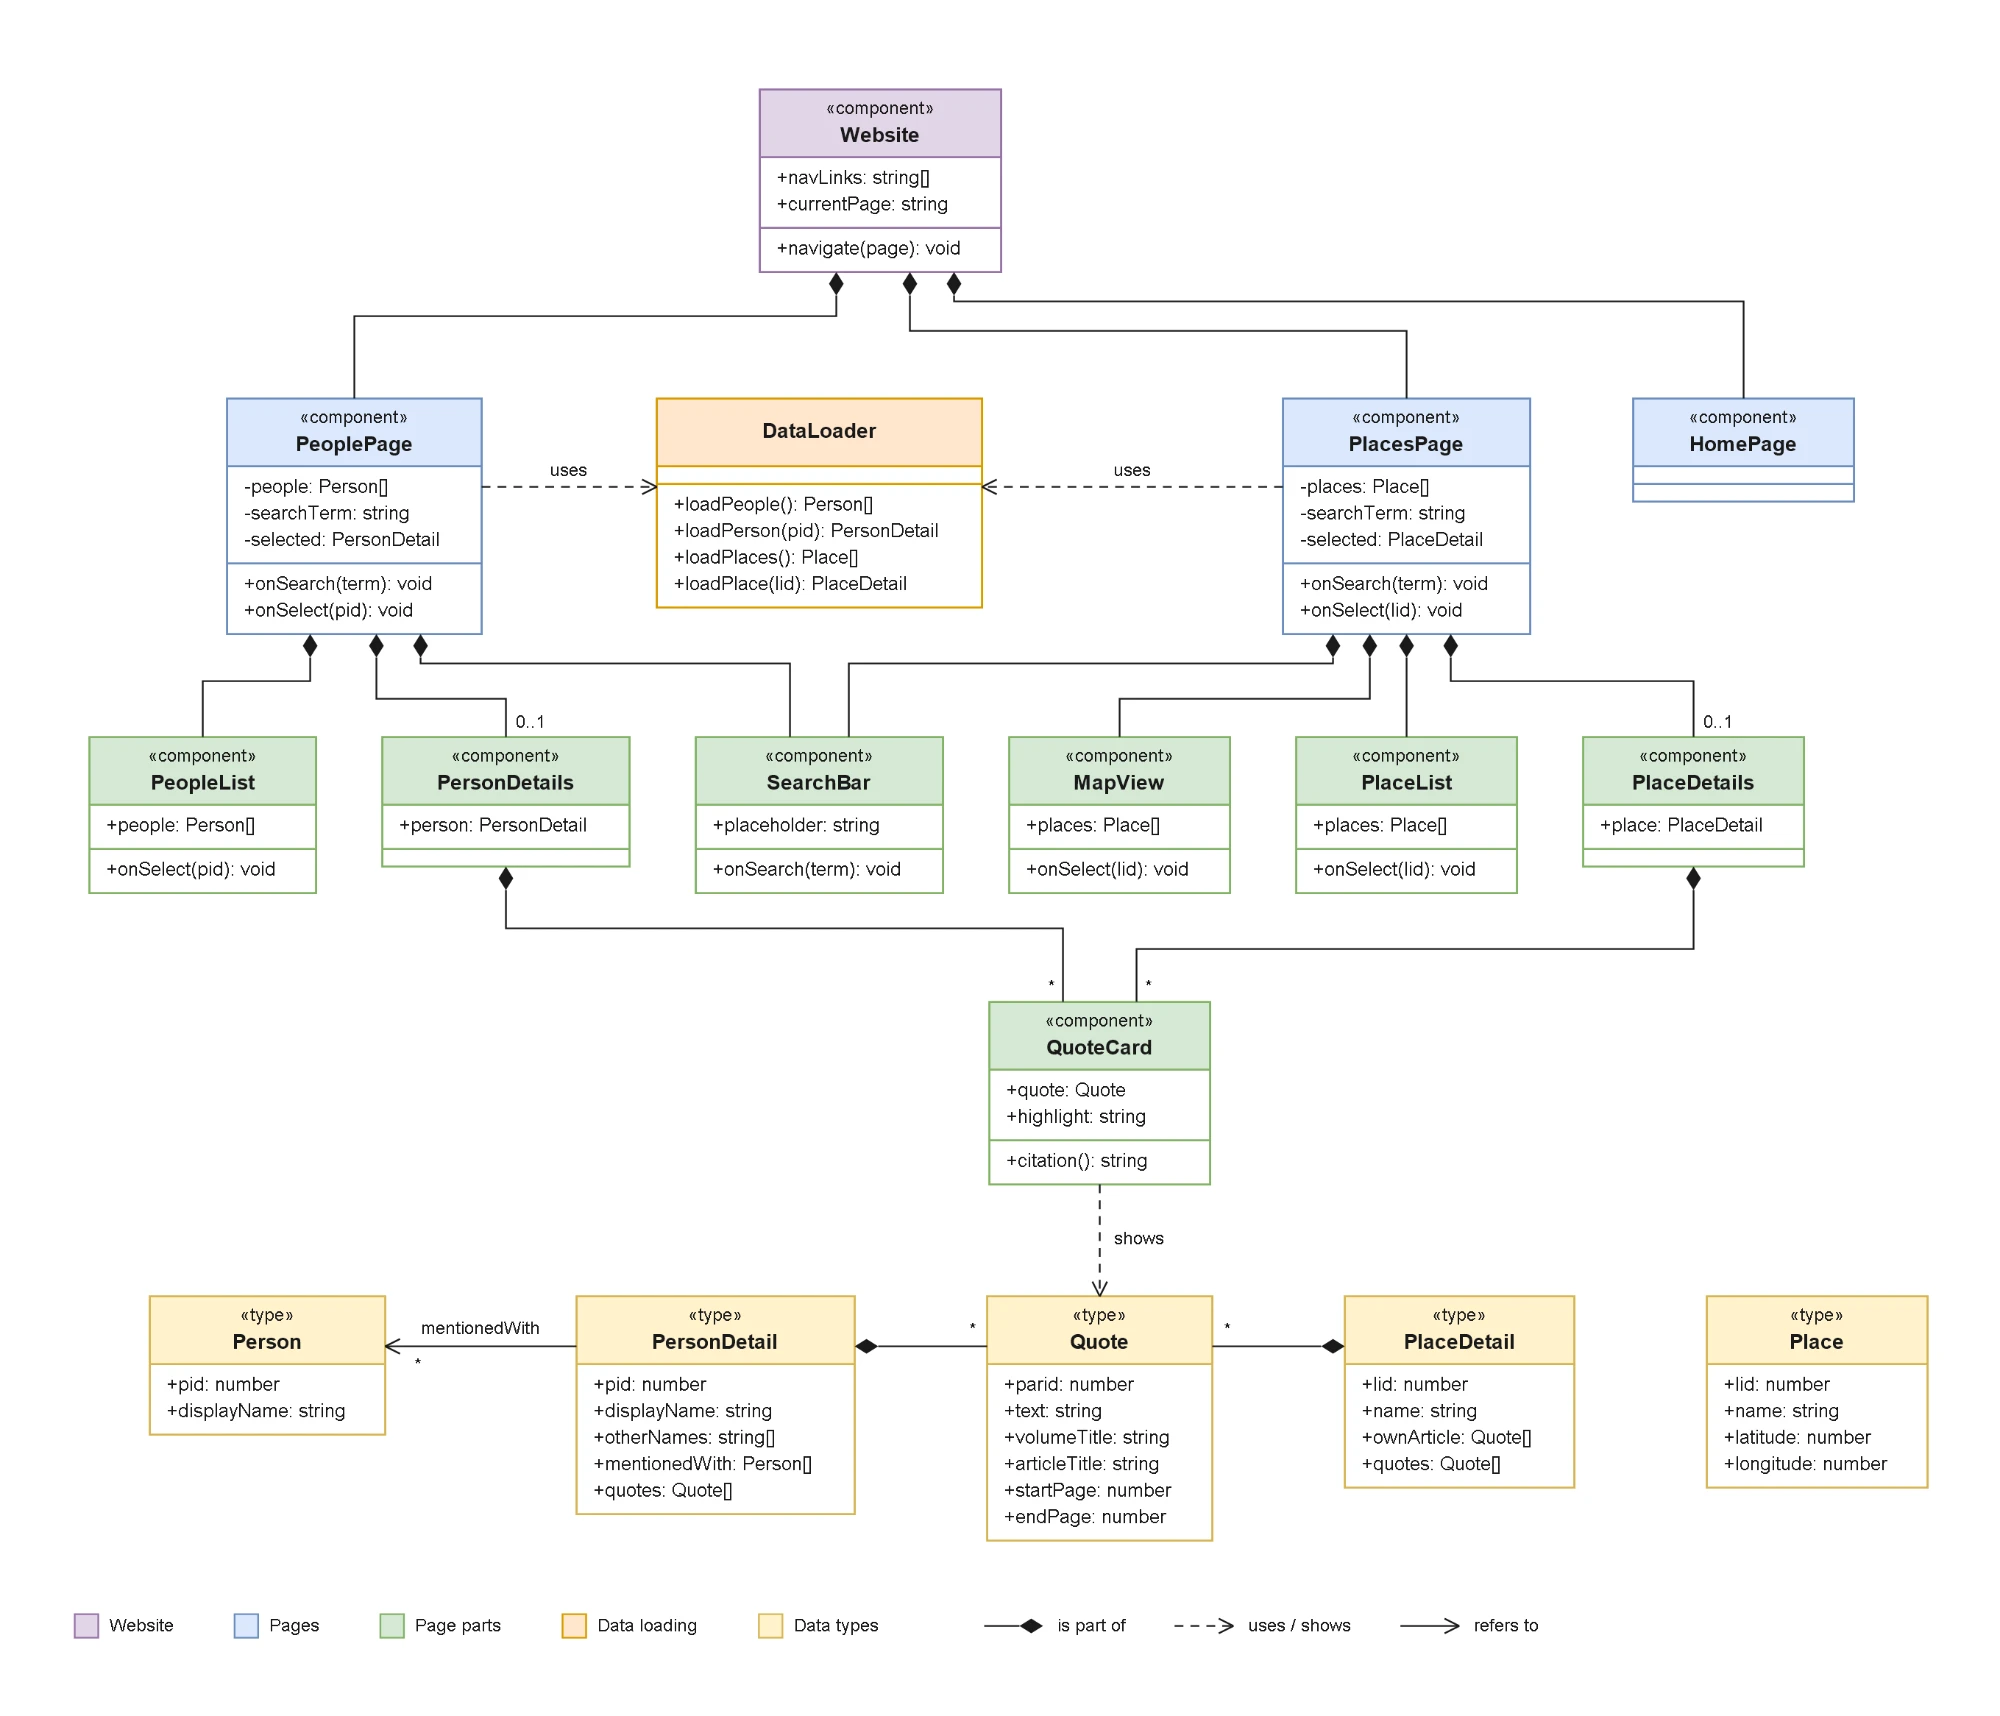
\includegraphics[width=\linewidth,height=0.6\textheight,keepaspectratio]{class-frontend}
  \caption{Front end class diagram}
\end{figure}

% ---------------------------------------------------------------- 7
\clearpage
\section{Block Diagram}\label{sec:block}

The block diagram is the architecture deliverable. It shows the four major
components of the system and the data passed between them.

\begin{itemize}
  \item The \textbf{Web Scraper} saves the encyclopedia to the
        \textbf{Database} and passes it to the \textbf{NLP} component as input.
  \item The \textbf{NLP} component processes the text and saves the resulting
        relational tree to the \textbf{Database}.
  \item The \textbf{Website} requests relational data from the
        \textbf{Database}, which fulfills those requests.
\end{itemize}

The Database is the only component that both the processing side and the
website use, which keeps the website independent of when processing runs.

\begin{figure}[H]
  \centering
  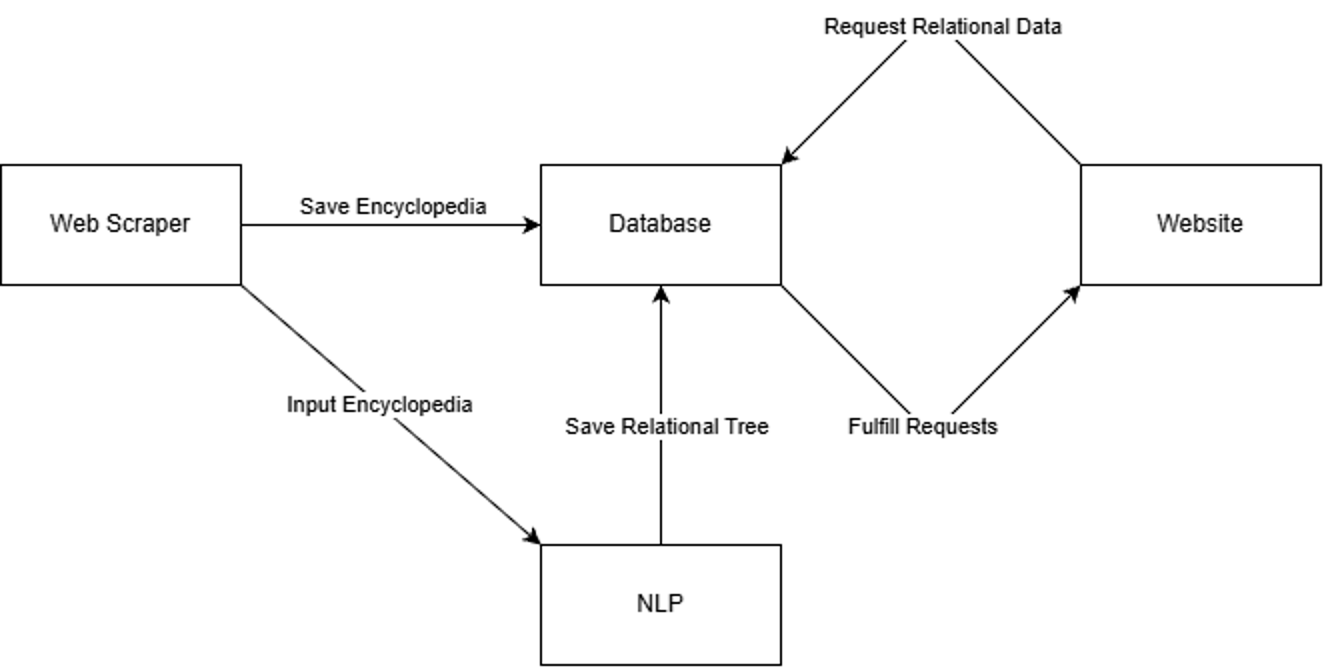
\includegraphics[width=\linewidth,height=0.5\textheight,keepaspectratio]{block}
  \caption{System architecture block diagram}
\end{figure}

% ---------------------------------------------------------------- 8
\clearpage
\section{Database Schema}\label{sec:schema}

The schema is a supplementary model showing how the project database stores the
records described by the domain model. Tables are grouped into three areas.

\begin{itemize}
  \item \textbf{Encyclopedia tables.} \texttt{Volume}, \texttt{Article}, and
        \texttt{Paragraph} store the source text. Each paragraph stores its
        position within its article and its start and end pages, and a unique
        index on article and position keeps paragraphs in order.
  \item \textbf{Places tables.} \texttt{Places} stores each location with its
        type, country, and coordinates. \texttt{Where\_\allowbreak Place\_\allowbreak Mentioned} links
        places to the paragraphs that mention them.
  \item \textbf{People tables.} \texttt{People} stores each person, and
        \texttt{Name\_Entry} stores every name under which a person is listed.
        \texttt{Where\_\allowbreak Person\_\allowbreak Mentioned} links people to the paragraphs that
        mention them.
\end{itemize}

Both mention tables use the paragraph and the person or place as a composite
primary key, so each person or place is recorded at most once per paragraph.
Additional indexes support searching by name and building each person's and
place's page.

\begin{figure}[H]
  \centering
  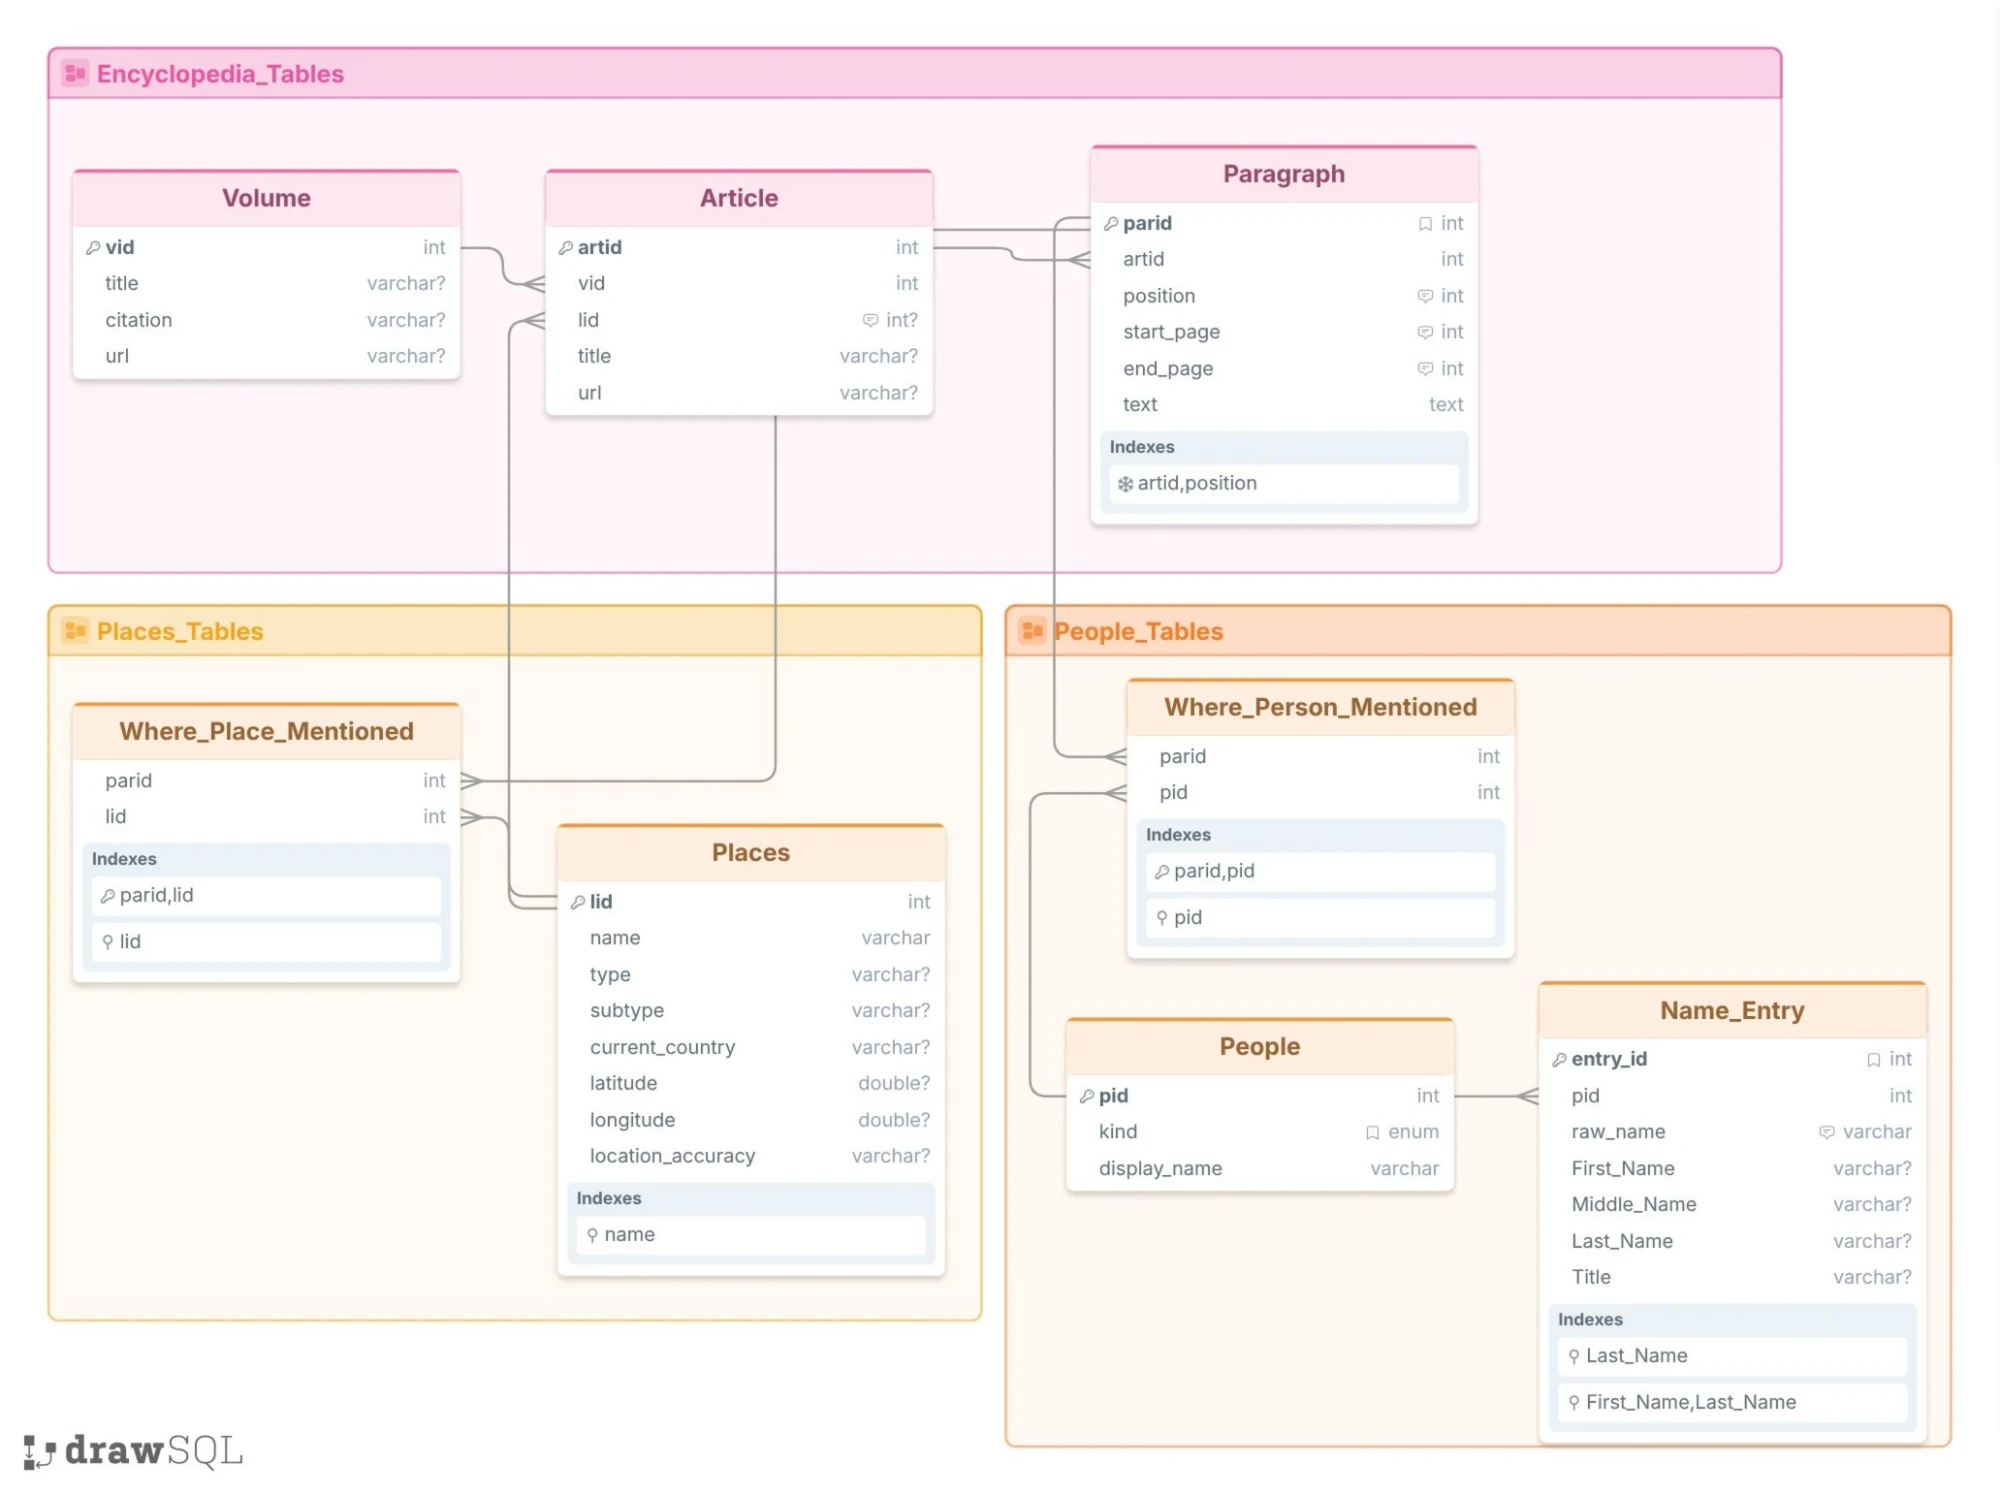
\includegraphics[width=\linewidth,height=0.6\textheight,keepaspectratio]{schema}
  \caption{Database schema}
\end{figure}

\end{document}
